\chapter{有时候,精英主义是可以接受的}\label{chap:w4}

\noindent \href{https://github.com/taseikyo/arts}{readme} | \hyperref[chap:w3]{previous} | \hyperref[chap:w5]{next}

\begin{figure}[htbp]
  \centering
    
\includegraphics[width=\textwidth]{../images/2020/11/lala-azizli-OFZUaeYKP3k-unsplash.jpg}
  \caption{\textit{Photo by Lala Azizli on Unsplash}}
\end{figure}

\textit{总字数:2079 个(汉字:1278,英文单词:302,数字:79,中文标点:160,英文标点:260),阅读时长约:4 分 6 秒。}

\section{algorithm \hyperref[chap:w4]{top}}\label{w4:algorithm}

\subsection{\href{https://leetcode-cn.com/problems/gas-station/}{134.加油站}}

环路,N 个加油站,每个有汽油 gas[i] 升,从 i 到 i+1 消耗 cost[i],初始油箱为 0(容量无限),问从哪点出发能绕一圈,否则返回 0。

这个 \href{https://leetcode-cn.com/problems/gas-station/solution/shou-hua-tu-jie-liang-ge-guan-jian-jie-lun-de-jian/}{题解} 写的很清楚,只要总加油量比总耗油量大就一定有解,关键在于找到出发点。

\begin{figure}[htbp]
  \centering
    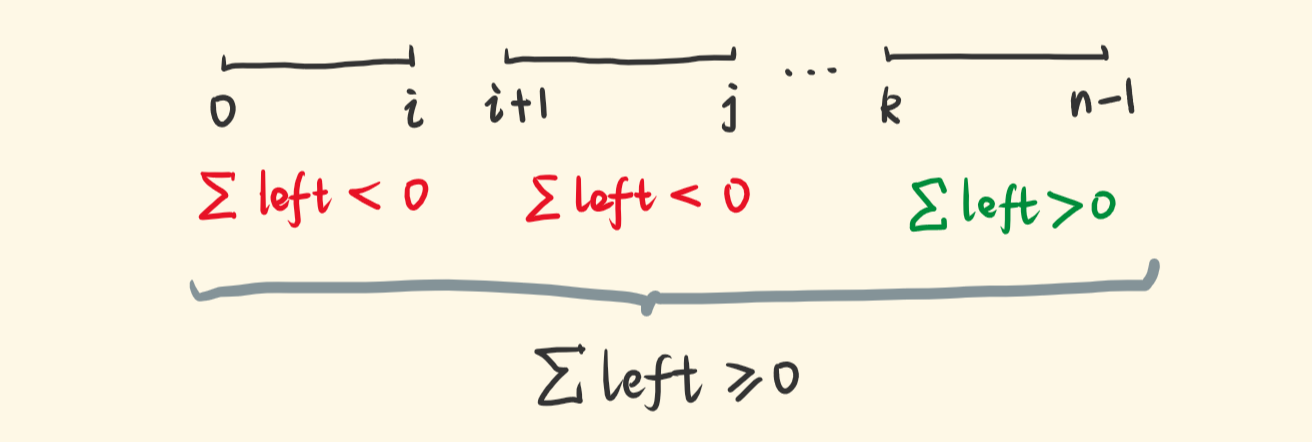
\includegraphics[width=\textwidth]{../images/2020/11/w4-algo-1.png}
  \caption{\textit{w4-algo-1.png}}
\end{figure}

上图中,若从 0 出发到 i 的剩余油量小于 0,那么 0 \textasciitilde i 都不能作为起点,类似地 i+1 \textasciitilde j 也不能,由于总剩余为正,那么必然有一段为正,图中 k 就为起点,后面一段能加到足够的油补充前面两段不足,从而绕一圈。

简单说明一下 0 \textasciitilde i 都不能作为起点的原因,比如 a-b-c-d,到 c 的时候剩余为负,此时我们能得到啥?

\begin{itemize}
\item 显然 a 是不能作为起点的:$ (gas[a]-cost[a])+(gas[b]-cost[b])+(gas[c]-cost[c])<0 => left(a)+left(b)+left(c)<0 $
\item 由于过了 a,所以 $ left(a) >= 0 => left(b)+left(c)<0 $,所以 b 也做不了起点
\item 同理能到 c 肯定过了 b,即,$ left(a)+left(b)>=0 => left(c)<0 $,所以 c 也做不了起点
\end{itemize}

\begin{itemize}
  \item \href{https://github.com/taseikyo/arts/blob/master/code/leetcode_0134.go}{code/leetcode\_0134.go}
\end{itemize}

\begin{lstlisting}[language=go]
func canCompleteCircuit(gas []int, cost []int) int {
	left := 0
	start := 0
	totalGas, totalCost := 0, 0
	for i := 0; i < len(gas); i++ {
		totalGas += gas[i]
		totalCost += cost[i]
		left += gas[i] - cost[i]
		if left < 0 {
			start = i + 1
			left = 0
		}
	}
	if totalGas < totalCost {
		return -1
	}
	// 总加油>=总耗油,必然有解。当遍历结束时,最新的start指向成功的起点
	return start
}
\end{lstlisting}

\section{review \hyperref[chap:w4]{top}}\label{w4:review}

\subsection{\href{https://thenewstack.io/which-programming-languages-use-the-least-electricity/}{哪种编程语言用电量最少?(英文)}}

很有趣的一篇文章,他们比较了 27 种编程语言的能耗、速度和内存情况。

可能我们的直觉来看编译型语言运行快,他们的能耗少,事实确实如此,但是没有一个语言能在三种情况中都居榜首,如下如所示,C 在内存方面被 Pascal 和 Go 打败了,这个我还挺奇怪的,我以为 C 会屠榜来着,但总的来说编译型快于虚拟机型快于解释型(图中 c 表示 compiled,i 表示 interpreted,v 表示 virtual machine)。

\begin{figure}[htbp]
  \centering
    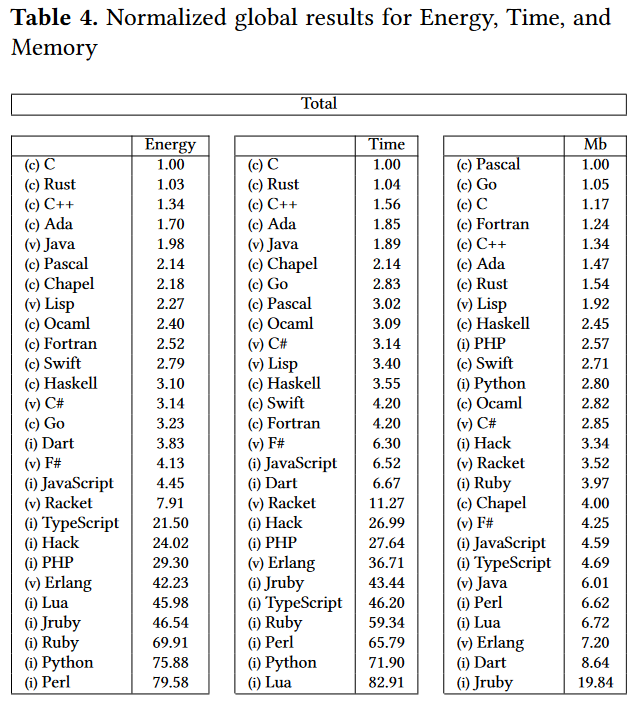
\includegraphics[width=0.6\textwidth]{../images/2020/11/w4-review-1.png}
  \caption{\textit{w4-review-1.png}}
\end{figure}

\section{tip \hyperref[chap:w4]{top}}\label{w4:tip}

\subsection{\href{https://stackoverflow.com/questions/2361426/get-the-first-item-from-an-iterable-that-matches-a-condition}{从(无穷)可迭代对象中获取匹配条件的第一项(StackOverflow)}}

简单一点我们可以这样做:

\begin{lstlisting}[language=Python]
def first(the_iterable, condition=lambda x: True):
	for i in the_iterable:
		if condition(i):
			return i

>>> first(range(10))
0
>>> first(range(10), lambda i: i > 3)
4
\end{lstlisting}

但其实我们可以使用内置的 next 函数完成这件事,并且可以设置默认值:

\begin{lstlisting}[language=Python]
def first(the_iterable, condition=lambda x: True, default_value=0):
	return next((x for x in the_iterable if condition(x)), default_value)

>>> first(range(10))
0
>>> first(range(10), lambda i: i > 3)
4
>>> first(range(10), lambda i: i > 30, -1)
-1
\end{lstlisting}

\subsection{\href{https://blog.csdn.net/Cinderella___/article/details/88697062}{搭建最简单的 Windows http web 服务器(中文)}}

\href{http://www.rejetto.com/hfs/?f=dl}{HFS \textasciitilde Http File Server},一个很小的可执行文件,双击运行即可。hfs 对于需要一个临时的 web 服务器是一个不错的选择。

\begin{figure}[htbp]
  \centering
    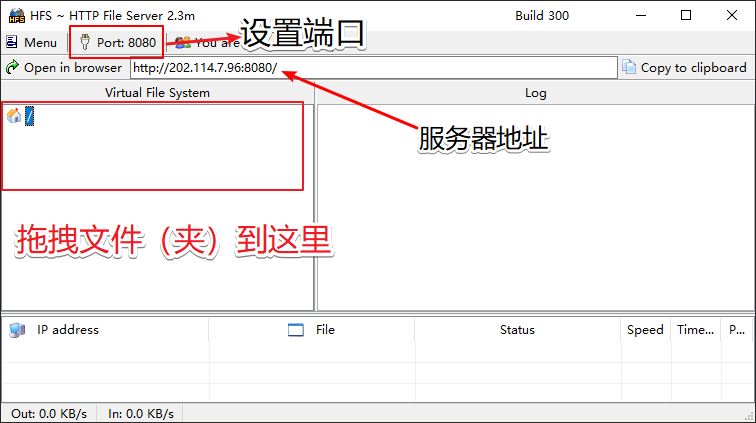
\includegraphics[width=0.8\textwidth]{../images/2020/11/Snipaste_20201116_210823.png}
  \caption{\textit{Snipaste\_20201116\_210823.png}}
\end{figure}

\subsection{\href{https://www.jianshu.com/p/7f4572b88c84}{git commit 格式正确书写方式(中文)}}

正如我做了 Markdown 的约定一样,git commit 也得有个约定,不然每次书写都以不同格式写看得人眼花缭乱,所以搜了一下,这篇文章写得挺简单,够我使用了。

格式:

\begin{lstlisting}[language=Bash]
<type>(scope): desc
\end{lstlisting}

\begin{itemize}
\item type 用来说明类型,常用的有以下几种:
  \begin{itemize}
    \item feat:完成新功能的开发
    \item fix:代码 BUG 的修复
    \item style:样式的修改
    \item refactor:代码重构
    \item docs:文档
    \item chore:构建工具
  \end{itemize}
\item scope 用来说明此次变动影响的范围或文件
\item desc 用来简短描述此次的变动,描述只要简明易理解就好,没必要写很多
\end{itemize}

如:\lstinline{feat(deployment.js): add app deploy function}

\section{share \hyperref[chap:w4]{top}}\label{w4:share}

\subsection{\href{https://www.arp242.net/elitist.html}{有时候,精英主义是可以接受的(英文)}}

\textit{It's fine to be elitist, sometimes},作者写这篇文章的起因是他参加一个 go 测试风格的会议并做报告,结果会上有个不会 go 的人一直提问 go 的基本语法,使得作者很恼火,作者认为与会人员应对 go 有基本了解。这个其实很多人深有体会,一图以蔽之:

\begin{figure}[htbp]
  \centering
    
\includegraphics[width=\textwidth]{../images/2020/11/w4-share-1.jpg}
  \caption{\textit{你不会百度吗?}}
\end{figure}

没有人有义务为你解释基本的东西,这些明明自己动动手就能查到,也许别人心情好会解释给你,但是别人并不总是闲的,正如作者所言:\textit{I will gladly go out of my way to try and explain things to new programmers. But not always, not at every place. I want to do it on my terms, when I feel like it, and reject that I have an obligation to do so all the time.}

毕竟对于要讨论的话题,你跟一个很/有所了解的人,跟一个完全不了解的人交谈是完全不同的,与后者肯定很费劲,你需要解释很多基本概念;但是与前者交流就很愉悦,或许对某个点更深入理解,或许对一个点颠覆认知(横看成岭侧成峰,每个人看待事物角度跟方式不同)。所以作者说有时候,精英主义是可以接受的,有些社区就是为专业人士设立的,新手还是不要一头撞进去,比如你想为开源社区做贡献,你可以先尝试为一些简单的项目修修 bug,不要一上来就想为 Linux 贡献代码,当然对于大佬这句话当我没说。

怎么说呢,我自己也是深有体会,进大学对计算机是一片空白,编程啥也不懂,也不会搜索引擎的一些技巧,开始也会问白痴问题,后来也就学会自己动手,慢慢积累基础嘛。如果实在查不到(应该是少数),再去问别人,这样过滤了大量基本辣鸡问题,对于难处理的问题别人或许会更容易接受一些,至少我是这么觉得。

很简单的一个例子,两个问题:

\begin{enumerate}
\item vector 怎么遍历/插入/删除元素?
\item vector 怎么边遍历边删除元素?
\end{enumerate}

我可能更乐意回复第二个问题,第一个我可能会说去百度吧;

\noindent \href{https://github.com/taseikyo/arts}{readme} | \hyperref[chap:w3]{previous} | \hyperref[chap:w5]{next}
